% Compile with: uplatex file.tex && dvipdfmx file.dvi
%           or: latexmk -uplatex file.tex
%\documentclass[uplatex,dvipdfmx]{jsarticle}
\documentclass[dvipdfmx,a4paper,11pt]{jsarticle}
\usepackage{amsmath, amssymb}
\usepackage{tikz}

\title{scenario\_notation\_regression}
\date{\today}

\begin{document}
\maketitle

記法の回帰確認。一度壊れていた綴りを毎回打ち直し、意味が変わらないことを実例の差分で見る。

A をベクトル場とする

\[
  A
\]

f をスカラー場とする

\[
  f
\]

$\psi_\sigma$

\begin{equation}
  \psi_\sigma
  \label{eq:E1}
\end{equation}

E1 を簡約して

\begin{equation}
  \psi_{\sigma}
  \label{eq:E2}
\end{equation}

G(t, t')

\begin{equation}
  G(t, t')
  \label{eq:E3}
\end{equation}

E3 を簡約して

\begin{equation}
  G\left(t , t'\right)
  \label{eq:E4}
\end{equation}

$\mathbf r$

\begin{equation}
  \mathbf r
  \label{eq:E5}
\end{equation}

E5 を簡約して

\begin{equation}
  \mathbf{r}
  \label{eq:E6}
\end{equation}

$\vec{A}(t)$

\begin{equation}
  \vec{A}(t)
  \label{eq:E7}
\end{equation}

$\nabla \times \vec{A}$

\begin{equation}
  \left[ \frac{d}{d y} A_{z}-\frac{d}{d z} A_{y} , \frac{d}{d z} A_{x}-\frac{d}{d x} A_{z} , \frac{d}{d x} A_{y}-\frac{d}{d y} A_{x} \right]
  \label{eq:E8}
\end{equation}

$\nabla \cdot \vec{A}$

\begin{equation}
  \frac{d}{d z} A_{z}+\frac{d}{d y} A_{y}+\frac{d}{d x} A_{x}
  \label{eq:E9}
\end{equation}

$\nabla \vec{f}$

\begin{equation}
  \left[ \frac{d}{d x} f , \frac{d}{d y} f , \frac{d}{d z} f \right]
  \label{eq:E10}
\end{equation}

$\vec{A}$ の回転を求めて

\begin{equation}
  \vec{A}
  \label{eq:E11}
\end{equation}

\begin{equation}
  \left[ \frac{d}{d y} A_{z}-\frac{d}{d z} A_{y} , \frac{d}{d z} A_{x}-\frac{d}{d x} A_{z} , \frac{d}{d x} A_{y}-\frac{d}{d y} A_{x} \right]
  \label{eq:E12}
\end{equation}

$\lim_{x \to 0} \frac{\sin x}{x}$

\begin{equation}
  \lim_{x \to 0} \frac{\sin x}{x}
  \label{eq:E13}
\end{equation}

E13 を簡約して

\begin{equation}
  1
  \label{eq:E14}
\end{equation}

$\lim_{x \to 0^+} \frac{1}{x}$

\begin{equation}
  \lim_{x \to 0^+} \frac{1}{x}
  \label{eq:E15}
\end{equation}

E15 を簡約して

\begin{equation}
  \infty
  \label{eq:E16}
\end{equation}

$\lim_{t' \to t^+} G(t,t')$

\begin{equation}
  \lim_{t' \to t^+} G(t,t')
  \label{eq:E17}
\end{equation}

$y = x^3$

\begin{equation}
  y = x^3
  \label{eq:E18}
\end{equation}

E18 を x で3階微分して

\begin{equation}
  \frac{d^{3}y}{dx^{3}} = 6
  \label{eq:E19}
\end{equation}

D = $\begin{pmatrix}$ 2 \& 1 \textbackslash{}\textbackslash{} 1 \& 2 $\end{pmatrix}$

\begin{equation}
  D = \begin{pmatrix} 2 & 1 \\ 1 & 2 \end{pmatrix}
  \label{eq:E20}
\end{equation}

[4, 0; 0, 1] の行列式を求めて

\begin{equation}
  \begin{pmatrix} 4 & 0 \\ 0 & 1 \end{pmatrix}
  \label{eq:E21}
\end{equation}

\begin{equation}
  4
  \label{eq:E22}
\end{equation}

A のノルムを求めて

\begin{equation}
  \sqrt{A_{z}^2+A_{y}^2+A_{x}^2}
  \label{eq:E23}
\end{equation}

f を x で偏微分して

\begin{equation}
  \frac{d}{d x} f
  \label{eq:E24}
\end{equation}

p を q の共役運動量とみなす

正準座標対 (q, p) を登録しました。以後「f と g のポアソン括弧を求めて」で利用できます。

q と p のポアソン括弧を求めて

\begin{equation}
  1
  \label{eq:E25}
\end{equation}

x のラプラス変換を X と宣言する

\begin{equation}
  X(s) = \int_0^{\infty} x(t)\, e^{-s t}\, dt
  \label{eq:E26}
\end{equation}

$w = a v + b$

\begin{equation}
  w = a v + b
  \label{eq:E27}
\end{equation}

$v = 2 t$

\begin{equation}
  v = 2 t
  \label{eq:E28}
\end{equation}

E27 に E28 を置換して

\begin{equation}
  w = 2 a t+b
  \label{eq:E29}
\end{equation}

E27 の v に 5 を置き換えて

\begin{equation}
  w = b+5 a
  \label{eq:E30}
\end{equation}

$u + z = 3$

\begin{equation}
  u + z = 3
  \label{eq:E31}
\end{equation}

$u - z = 1$

\begin{equation}
  u - z = 1
  \label{eq:E32}
\end{equation}

u と z について E31 と E32 を解いて

\begin{equation}
  u = 2
  \label{eq:E33}
\end{equation}

\begin{equation}
  z = 1
  \label{eq:E34}
\end{equation}

$s = x^5$

\begin{equation}
  s = x^5
  \label{eq:E35}
\end{equation}

E35 を x で2階偏微分して

\begin{equation}
  \frac{\partial^{2} s}{\partial x^{2}} = 20 x^3
  \label{eq:E36}
\end{equation}

$\nabla \times \vec{A}$

\begin{equation}
  \left[ \frac{d}{d y} A_{z}-\frac{d}{d z} A_{y} , \frac{d}{d z} A_{x}-\frac{d}{d x} A_{z} , \frac{d}{d x} A_{y}-\frac{d}{d y} A_{x} \right]
  \label{eq:E37}
\end{equation}

B をベクトル場とする

\[
  B
\]

$\vec{A}$ と $\vec{B}$ の内積を求めて

\begin{equation}
  A_{z} B_{z}+A_{y} B_{y}+A_{x} B_{x}
  \label{eq:E38}
\end{equation}

$\nabla$ $\times$ $\vec{A}$ と $\vec{B}$ の外積を求めて

\begin{equation}
  \left[ \left(\frac{d}{d z} A_{x}-\frac{d}{d x} A_{z}\right) B_{z}-\left(\frac{d}{d x} A_{y}-\frac{d}{d y} A_{x}\right) B_{y} , \left(\frac{d}{d x} A_{y}-\frac{d}{d y} A_{x}\right) B_{x}-\left(\frac{d}{d y} A_{z}-\frac{d}{d z} A_{y}\right) B_{z} , \left(\frac{d}{d y} A_{z}-\frac{d}{d z} A_{y}\right) B_{y}-\left(\frac{d}{d z} A_{x}-\frac{d}{d x} A_{z}\right) B_{x} \right]
  \label{eq:E39}
\end{equation}

$\nabla \cdot (\nabla \times \vec{A})$

\begin{equation}
  0
  \label{eq:E40}
\end{equation}

A の回転の回転を求めて

\begin{equation}
  \left[ \frac{d^2}{d x d z} A_{z}+\frac{d^2}{d x d y} A_{y}-\frac{d^2}{d z^2} A_{x}-\frac{d^2}{d y^2} A_{x} , \frac{d^2}{d y d z} A_{z}-\frac{d^2}{d z^2} A_{y}-\frac{d^2}{d x^2} A_{y}+\frac{d^2}{d x d y} A_{x} , -\left(\frac{d^2}{d y^2} A_{z}\right)-\frac{d^2}{d x^2} A_{z}+\frac{d^2}{d y d z} A_{y}+\frac{d^2}{d x d z} A_{x} \right]
  \label{eq:E41}
\end{equation}

$\nabla s$

\begin{equation}
  \left[ 5 x^4 , 0 , 0 \right]
  \label{eq:E42}
\end{equation}

s のラプラシアンを求めて

\begin{equation}
  20 x^3
  \label{eq:E43}
\end{equation}

$P = [0, x, 0]$

\begin{equation}
  P = [0, x, 0]
  \label{eq:E44}
\end{equation}

2 P の回転を求めて

\begin{equation}
  2 P
  \label{eq:E45}
\end{equation}

\begin{equation}
  \left[ 0 , 0 , 2 \right]
  \label{eq:E46}
\end{equation}

P + 2 B の発散を求めて

\begin{equation}
  P + 2 B
  \label{eq:E47}
\end{equation}

\begin{equation}
  2 \left(\frac{d}{d z} B_{z}\right)+2 \left(\frac{d}{d y} B_{y}\right)+2 \left(\frac{d}{d x} B_{x}\right)
  \label{eq:E48}
\end{equation}

$\vec{P}$ $\times$ $\vec{A}$ の発散を求めて

\begin{equation}
  \vec{P} \times \vec{A}
  \label{eq:E49}
\end{equation}

\begin{equation}
  \frac{d}{d x} A_{z} x-\frac{d}{d z} A_{x} x+A_{z}
  \label{eq:E50}
\end{equation}

$Q = [z, 0, y]$

\begin{equation}
  Q = [z, 0, y]
  \label{eq:E51}
\end{equation}

2 ($\vec{P}$ $\times$ $\vec{Q}$) の発散を求めて

\begin{equation}
  2 (\vec{P} \times \vec{Q})
  \label{eq:E52}
\end{equation}

\begin{equation}
  2 y-2 x
  \label{eq:E53}
\end{equation}

$\vec{P}$ $\times$ $\vec{Q} + \vec{A}$ の発散を求めて

\begin{equation}
  \vec{P} \times \vec{Q} + \vec{A}
  \label{eq:E54}
\end{equation}

\begin{equation}
  y-x+\frac{d}{d z} A_{z}+\frac{d}{d y} A_{y}+\frac{d}{d x} A_{x}
  \label{eq:E55}
\end{equation}

a $x^2$ を x で積分して

\begin{equation}
  a x^2
  \label{eq:E56}
\end{equation}

\begin{equation}
  \int a x^2 \, dx = \frac{a x^3}{3} + C
  \label{eq:E57}
\end{equation}

a $x^2$ を x で全微分して

\begin{equation}
  \frac{d}{dx}\left(a x^2\right) = 2 a x
  \label{eq:E58}
\end{equation}

$K = 3 (\vec{P} \times \vec{Q})$

\begin{equation}
  K = 3 (\vec{P} \times \vec{Q})
  \label{eq:E59}
\end{equation}

K を簡約して

\begin{equation}
  K = \left[ 3 x^4 , 0 , -\left(3 x\right) \right]
  \label{eq:E60}
\end{equation}

$m^2 + 3$

\begin{equation}
  m^2 + 3
  \label{eq:E61}
\end{equation}

$2 m = 8$

\begin{equation}
  2 m = 8
  \label{eq:E62}
\end{equation}

E62 を m について解いて

\begin{equation}
  m = 4
  \label{eq:E63}
\end{equation}

E61 を m で全微分して

\begin{equation}
  \frac{d}{dm}\left(m^2 + 3\right) = 2 m
  \label{eq:E64}
\end{equation}

E61 を m で積分して

\begin{equation}
  \int m^2 + 3 \, dm = \frac{m^3}{3}+3 m + C_1
  \label{eq:E65}
\end{equation}

$\bar{y}^2 + t'$

\begin{equation}
  \bar{y}^2 + t'
  \label{eq:E66}
\end{equation}

E66 を $\bar{y}$ で偏微分して

\begin{equation}
  \frac{\partial}{\partial \bar{y}}\left(\bar{y}^2 + t'\right) = 2 \bar{y}
  \label{eq:E67}
\end{equation}

E66 を t' で偏微分して

\begin{equation}
  \frac{\partial}{\partial t'}\left(\bar{y}^2 + t'\right) = 1
  \label{eq:E68}
\end{equation}

E66 を $\bar{y}$ で積分して

\begin{equation}
  \int \bar{y}^2 + t' \, d\bar{y} = \frac{\bar{y}^3}{3}+t' \bar{y} + C_2
  \label{eq:E69}
\end{equation}

$\int r^2 \, dr$

\begin{equation}
  \int r^2 \, dr
  \label{eq:E70}
\end{equation}

E70 の r を u に変数変換して

\begin{equation}
  \int {u^2}{\;du}
  \label{eq:E71}
\end{equation}

$\alpha + \beta = 3$

\begin{equation}
  \alpha + \beta = 3
  \label{eq:E72}
\end{equation}

$\alpha - \beta = 1$

\begin{equation}
  \alpha - \beta = 1
  \label{eq:E73}
\end{equation}

E72 と E73 を $\alpha$ と $\beta$ について解いて

\begin{equation}
  \alpha = 2
  \label{eq:E74}
\end{equation}

\begin{equation}
  \beta = 1
  \label{eq:E75}
\end{equation}

$Sz_i$ $Sz_j$ の隣接和を 4 サイト 周期境界で展開して

\begin{equation}
  Sz\left(3\right) Sz\left(4\right)+Sz\left(1\right) Sz\left(4\right)+Sz\left(2\right) Sz\left(3\right)+Sz\left(1\right) Sz\left(2\right)
  \label{eq:E76}
\end{equation}

\begin{center}
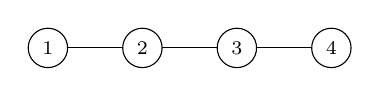
\begin{tikzpicture}[scale=1.2, site/.style={circle,draw,fill=white,inner sep=1pt,minimum size=5mm,font=\scriptsize}]
  \draw (0.000,0.000) -- (1.000,0.000);
  \draw (1.000,0.000) -- (2.000,0.000);
  \draw (2.000,0.000) -- (3.000,0.000);
  \draw[dashed] (3.000,0.000) -- (0.000,0.000);
  \node[site] at (0.000,0.000) {1};
  \node[site] at (1.000,0.000) {2};
  \node[site] at (2.000,0.000) {3};
  \node[site] at (3.000,0.000) {4};
\end{tikzpicture}
\end{center}

$Sz_i$ $Sz_j$ のハニカム格子 3x3 の格子和を展開して

\begin{equation}
  Sz\left(8\right) Sz\left(9\right)+Sz\left(7\right) Sz\left(8\right)+Sz\left(5\right) Sz\left(8\right)+Sz\left(5\right) Sz\left(6\right)+Sz\left(3\right) Sz\left(6\right)+Sz\left(4\right) Sz\left(5\right)+Sz\left(1\right) Sz\left(4\right)+Sz\left(2\right) Sz\left(3\right)+Sz\left(1\right) Sz\left(2\right)
  \label{eq:E77}
\end{equation}

\begin{center}
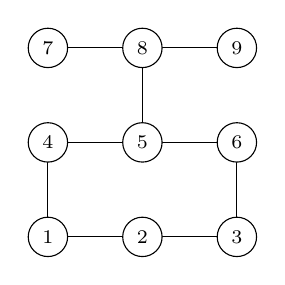
\begin{tikzpicture}[scale=1.2, site/.style={circle,draw,fill=white,inner sep=1pt,minimum size=5mm,font=\scriptsize}]
  \draw (0.000,0.000) -- (1.000,0.000);
  \draw (1.000,0.000) -- (2.000,0.000);
  \draw (0.000,1.000) -- (1.000,1.000);
  \draw (1.000,1.000) -- (2.000,1.000);
  \draw (0.000,2.000) -- (1.000,2.000);
  \draw (1.000,2.000) -- (2.000,2.000);
  \draw (0.000,0.000) -- (0.000,1.000);
  \draw (1.000,1.000) -- (1.000,2.000);
  \draw (2.000,0.000) -- (2.000,1.000);
  \node[site] at (0.000,0.000) {1};
  \node[site] at (1.000,0.000) {2};
  \node[site] at (2.000,0.000) {3};
  \node[site] at (0.000,1.000) {4};
  \node[site] at (1.000,1.000) {5};
  \node[site] at (2.000,1.000) {6};
  \node[site] at (0.000,2.000) {7};
  \node[site] at (1.000,2.000) {8};
  \node[site] at (2.000,2.000) {9};
\end{tikzpicture}
\end{center}

$y'^3$

\begin{equation}
  y'^3
  \label{eq:E78}
\end{equation}

E78 を y' で微分して

\begin{equation}
  \frac{d}{dy'}\left(y'^3\right) = 3 y'^2
  \label{eq:E79}
\end{equation}

$2 (x)^3$

\begin{equation}
  2 (x)^3
  \label{eq:E80}
\end{equation}

E80 を簡約して

\begin{equation}
  2 x^3
  \label{eq:E81}
\end{equation}

$2^2 (x)$

\begin{equation}
  2^2 (x)
  \label{eq:E82}
\end{equation}

E82 を簡約して

\begin{equation}
  4 x
  \label{eq:E83}
\end{equation}

\end{document}